\apendice{Documentación técnica de programación}

\section{Introducción}

En el siguiente anexo se explica todo lo que tiene que conocer el programador para instalar el entorno de trabajo y poder seguir con el desarrollo de la aplicación.

\section{Estructura de directorios}

A continuación se explicará cada uno de los directorios de la aplicación con una pequeña explicación que facilite al siguiente desarrollador su entendimiento.

\dirtree{%
	.1 /.
	.2 Diseño/Diagramas \desc{Aquí se encuentran los diagramas utilizados para diseñar la base de datos}.
	.2 documentacion \desc{Estructura de directorios de la plantilla \LaTeX}.
	.3 img \desc{carpeta donde se almacenan las imágenes de la documentación}.
	.3 tex \desc{Ficheros $.tex$ a compilar}.
	.2 resources .
	.3 readme \desc{Logotipos utilizados en el README.md}.
	.3 weblectric\_logo \desc{Logotipo personalizado para la aplicación}.
	.2 web/instalaciones\_electricas \desc{Estructura raíz del proyecto desarrollado en \textit{CakePHP}}.
	.3 config \desc{Ficheros de configuración}.
	.4 app.php \desc{Fichero de configuración más importante. Aquí se establece el valor del \textit{debug} y la conexión con la base de datos entre otras cosas}.	
	.4 routes.php \desc{Lugar donde se declaran constantes globales para las rutas del proyecto}.
	.3 files \desc{Carpeta para almacenar archivos a utilizar en la aplicación}.
	.3 src \desc{Directorio donde se encuentra la lógica de la aplicación. Estructurada a través del patrón MVC}.
	.4 Controller \desc{Controladores de la aplicación}.
	.4 Model \desc{Modelos de la aplicación}.
	.4 Template \desc{Vistas de la aplicación}.
	.3 tmp \desc{Lugar en el que CakePHP almacena temporalmente la información}.
	.3 webroot \desc{Raíz de los documentos públicos de la aplicación}.
	.4 css \desc{Hojas de estilos de la aplicación}.
	.4 img \desc{Directorio donde clasificar las imágenes que se carguen en la aplicación}.
	.4 js \desc{Directorio para los ficheros escritos en \textit{Javascript}}.
	.2 README.md \desc{Descripción del proyecto}.
}


\section{Manual del programador}

En esta sección, se hablará de los puntos más importantes a tener en cuenta y de las aplicaciones necesarias con el objetivo de que en un futuro, un desarrollador pueda seguir trabajando en el proyecto. Todas las rutas expuestas a continuación, hacen referencia a un sistema operativo Windows.

\subsection{XAMPP}

En primer lugar, será necesario descargar \textit{XAMPP} en su versión 7.2.10. Su función es simular un servidor en un entorno de desarrollo local. Este paquete incluye las siguientes herramientas:

\begin{itemize}
	\item Apache 2.4.34
	\item MariaDB 10.1.36
	\item PHP 7.2.10
	\item phpMyAdmin 4.8.3
	\item OpenSSL 1.1.0g
\end{itemize}

La ventaja que proporciona la instalación de todas estas herramientas a través del paquete \href{https://www.apachefriends.org/es/index.html}{\textit{XAMPP}}\footnote{\textit{XAMPP}: \url{https://www.apachefriends.org/es/index.html}} es que la configuración ya viene hecha, no obstante, si el futuro desarrollador desea realizar la instalación y configuración de cada uno de los servicios por su cuenta en su máquina local, no hay ningún problema.

Si ejecutamos el archivo descargado, como podemos ver en la figura~\ref{img:XAMPP_Opciones}, nos dará a elegir entre qué servicios queremos instalar. El siguiente y último paso, figura~\ref{img:XAMPP_Ruta}, es indicar en qué ruta queremos realizar la instalación. 

\begin{figure}[h]
	\centering
	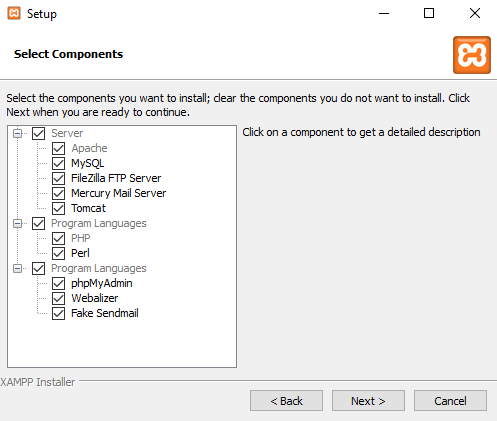
\includegraphics[width=1\textwidth]{/anexos/ManualProgramador/Xampp/1Opciones}
	\caption{\textit{XAMPP}: Servicios que se desean instalar.}
	\label{img:XAMPP_Opciones}
\end{figure}

\begin{figure}[h]
	\centering
	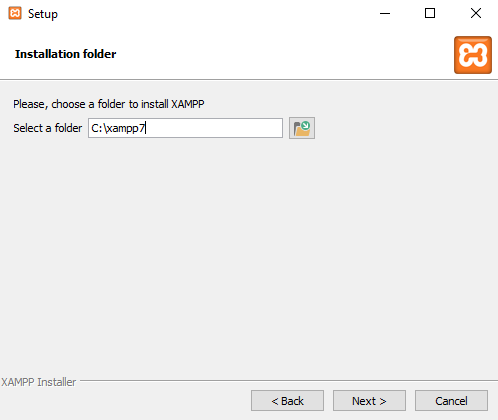
\includegraphics[width=1\textwidth]{/anexos/ManualProgramador/Xampp/2Ruta}
	\caption{\textit{XAMPP}: Ruta donde desplegarlo.}
	\label{img:XAMPP_Ruta}
\end{figure}

Para ver si se ha descargado e instalado correctamente, se puede ejecutar el siguiente comando con el que se mostrará por consola la versión del \textit{PHP} instalado:
\begin{lstlisting}[language=bash]
			php -v
\end{lstlisting}

Los resultados deben de ser como los que se muestran en la figura ~\ref{img:XAMPP_PHP_v}.

\begin{figure}[h]
	\centering
	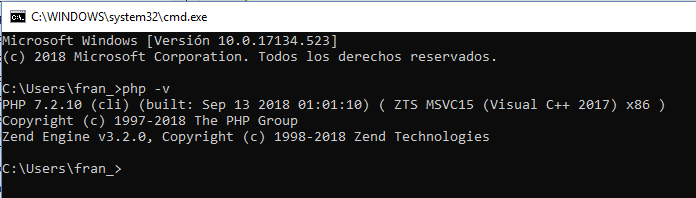
\includegraphics[width=1\textwidth]{/anexos/ManualProgramador/Xampp/3PhpVersion}
	\caption{\textit{XAMPP}: Resultado de ejecutar el comando $php -v$.}
	\label{img:XAMPP_PHP_v}
\end{figure}

Otra de las herramientas que presenta \textit{XAMPP} es un interesante panel de control como el de la figura~\ref{img:XAMPP_Panel}, en el que se podrá iniciar y apagar cada uno de los servicios.

\begin{figure}[h]
	\centering
	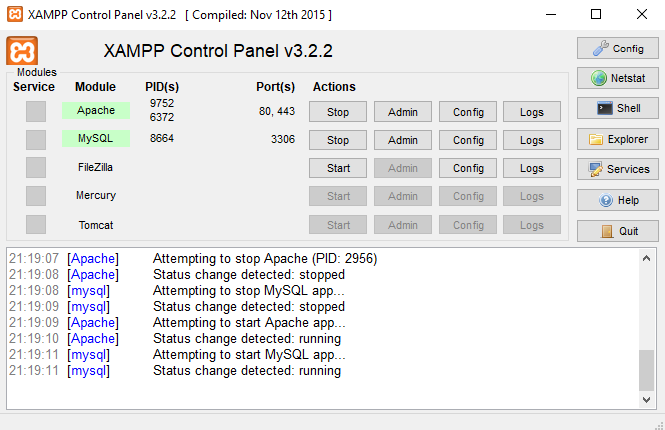
\includegraphics[width=1\textwidth]{/anexos/ManualProgramador/Xampp/4Panel}
	\caption{\textit{XAMPP}: Panel de control con \textit{Apache} y \textit{MySQL} iniciados.}
	\label{img:XAMPP_Panel}
\end{figure}

Si se inicia el servicio de \textit{Apache} correctamente, se puede ver que accediendo a la dirección \href{http://localhost}{localhost}\footnote{\url{http://localhost}} nos muestra información satisfactoria como la de la figura~\ref{img:XAMPP_Correct}.

\begin{figure}[h]
	\centering
	
\includegraphics[width=1\textwidth]{/anexos/ManualProgramador/Xampp/5CorrectInstallation}
	\caption{Mensaje de información acerca de que se ha instalado correctamente.}
	\label{img:XAMPP_Correct}
\end{figure}

Con \textit{XAMPP} funcionando, hay que configurar las direcciones para indicar dónde tenemos nuestro proyecto. Para ello habrá que cambiar alguna línea de código en el fichero de configuración $httpd.conf$ que se encuentra en la ruta \textit{\text{C:/xampp7/apache/conf}}.

Buscamos las líneas: 
\begin{lstlisting}[language=bash]
DocumentRoot "/xampp7/htdocs"
<Directory "/xampp7/htdocs">
\end{lstlisting}
y las cambiamos por la dirección donde hayamos colocado nuestro proyecto, en este caso: 
\begin{lstlisting}[language=bash]
DocumentRoot "C:\Users\fran_\Documents\GitHub\TFG-Instalaciones-Electricas\web\instalaciones_electricas"
<Directory "C:\Users\fran_\Documents\GitHub\TFG-Instalaciones-Electricas\web\instalaciones_electricas">
\end{lstlisting}

De esta manera, ya no redireccionará a la página anterior sino que cogerá la ruta especificada.

Aunque lo que se va a comentar a continuación no es obligatorio, si que es aconsejable pues si se desea tener varios proyectos, es incómodo trabajar con la dirección \textit{localhost}, pues tendríamos que andar modificando estos archivos continuamente. Para ello existe la posibilidad de configurar todos los \textit{virtual hosts} que se deseen. Esto significa que se podrán dar direcciones concretas a cada uno de los proyectos. Para ello, se descomentará la siguiente lnea:

\begin{lstlisting}[language=bash]
# Virtual hosts
Include conf/extra/httpd-vhosts.conf
\end{lstlisting}

El siguiente paso es dirigirse al fichero $httpd-vhosts.conf$ que se encuentra en el directorio \textit{\text{C:/xampp7/apache/conf/extra}} para colocar las siguientes lineas al final del archivo y crear un primer \textit{virtual hosts}.

\begin{lstlisting}[language=bash]
<VirtualHost *:80>
DocumentRoot "C:\Users\fran_\Documents\GitHub\TFG-Instalaciones-Electricas\web\instalaciones_electricas\webroot"
ServerName instalaciones_electricas.fsg
<Directory "C:\Users\fran_\Documents\GitHub\TFG-Instalaciones-Electricas\web\instalaciones_electricas\webroot">
Require all granted
</Directory>
</VirtualHost>
\end{lstlisting}

\begin{itemize}
\item \textit{DocumentRoot}: Aquí se indica la ruta del proyecto hasta la carpeta \textit{webroot}, que como se ha explicado antes es la parte pública a la que tiene acceso el usuario.
\item \textit{ServerName}: Dirección url para ese proyecto.
\end{itemize}

Cabe destacar que siempre que se modifique cualquier fichero de configuración se tendrán que reiniciar los servicios afectados, por lo que a continuación, el último paso será acceder de nuevo al panel de control~\ref{img:XAMPP_Panel} y reiniciar el servicio.

Por último, lo que queda de configurar es la base de datos \textit{MySQL}. Aunque con el paquete \textit{XAMPP} viene preparado para su uso desde \textit{phpMyAdmin}, se ha decidido descargar \href{https://www.heidisql.com/download.php}{\textit{HeidiSQL}}\footnote{\textit{HeidiSQL}: \url{https://www.heidisql.com/download.php}} pues presenta una interfaz más amigable y estable. Además, existe una versión portable que no requiere de instalación.

Si ejecutamos la aplicación, aparecerá una pantalla como la de la figura~\ref{img:Heidi}, donde nos aparecerán todas las sesiones que tengamos activas:

\begin{figure}[h]
	\centering
	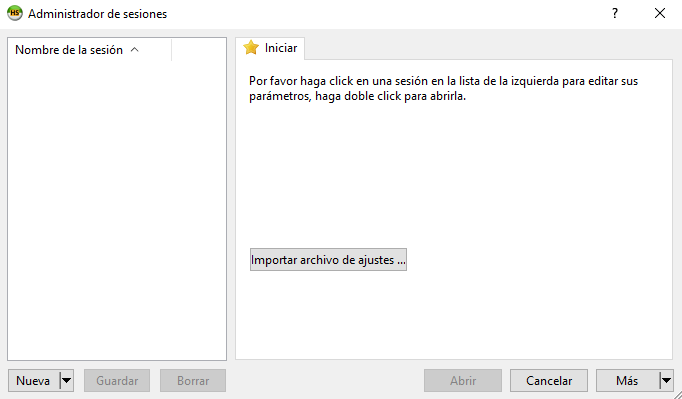
\includegraphics[width=1\textwidth]{/anexos/ManualProgramador/Xampp/8Heidi}
	\caption{Pantalla de inicio de \textit{HeidiSQL}.}
	\label{img:Heidi}
\end{figure}

Procedemos a crear una nueva sesión con los parámetros que se ven en la figura~\ref{img:Heidi_2}:

\begin{figure}[h]
	\centering
	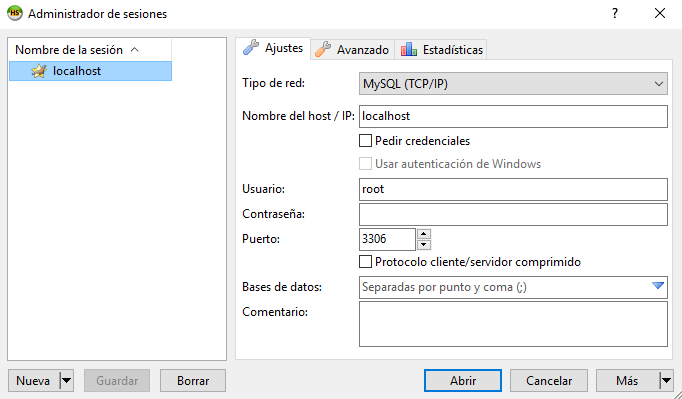
\includegraphics[width=0.9\textwidth]{/anexos/ManualProgramador/Xampp/9Heidi_2}
	\caption{Parámetros para una nueva sesión en entorno local.}
	\label{img:Heidi_2}
\end{figure}

Con la sesión ya creada, se podrá crear una base de datos nueva con las tabas que se desee. A continuación, en la figura~\ref{img:Heidi_3} se va a mostrar cómo crear un usuario para esa base de datos para que posteriormente se pueda enlazar con el proyecto. 

\begin{figure}[h]
	\centering
	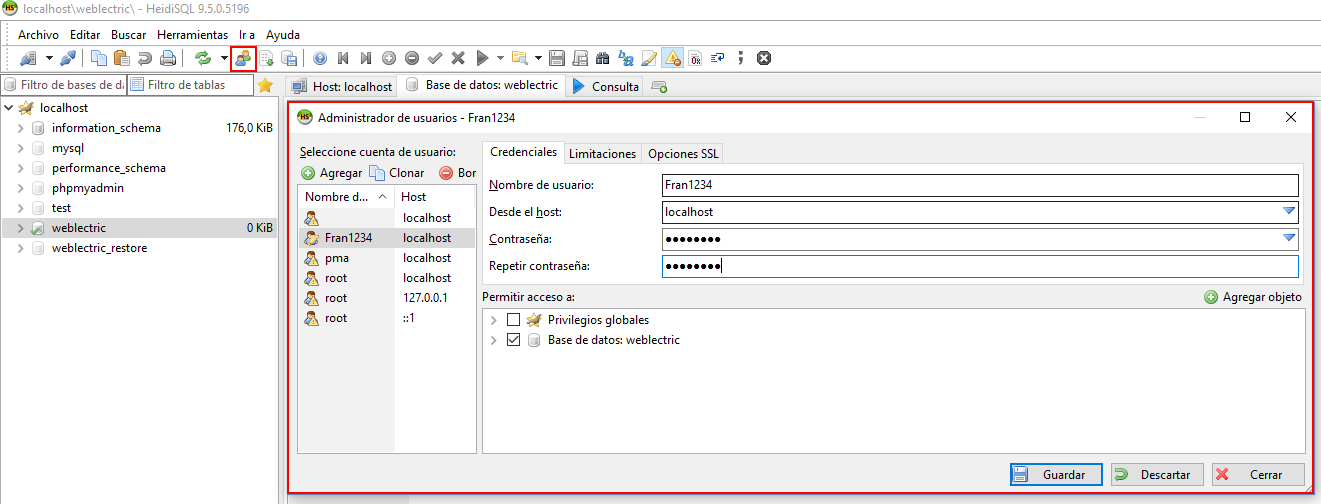
\includegraphics[width=0.9\textwidth]{/anexos/ManualProgramador/Xampp/10Heidi_3}
	\caption{Parámetros para asociar un usuario a la base de datos.}
	\label{img:Heidi_3}
\end{figure}

\newpage


\section{Compilación, instalación y ejecución del proyecto}

En primer lugar, se procederá a descargar \href{https://github.com/fransaiz95/Weblectric2018}{\textit{Weblectric}}\footnote{\textit{Weblectric}: \url{https://github.com/fransaiz95/Weblectric2018}} del repositorio de \textit{GitHub}.

El lugar en el que se descomprimirá el archivo descargado, será el directorio que se haya especificado anteriormente, en nuestro caso:
\begin{lstlisting}[language=bash]
C:\Users\fran_\Documents\GitHub\TFG-Instalaciones-Electricas\web\"
\end{lstlisting}

Como se puede ver en la figura~\ref{img:XAMPP_Finish}, si ahora se introduce la url que se ha establecido en el \textit{virtual host}, se accederá satisfactoriamente a la pantalla principal del proyecto.

\begin{figure}[h]
	\centering
	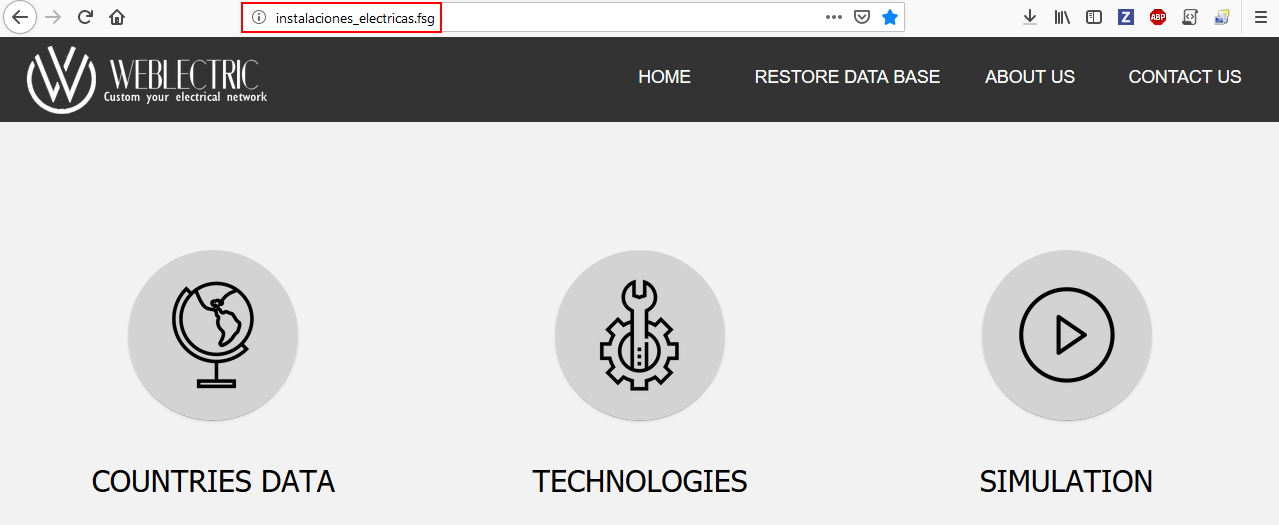
\includegraphics[width=1\textwidth]{/anexos/ManualProgramador/Xampp/6Finish}
	\caption{\textit{Virtual host} correctamente configurado.}
	\label{img:XAMPP_Finish}
\end{figure}

Dentro del entorno de desarrollo, no hay dificultades pues no hay más que abrir la carpeta contenedora del proyecto.

En este proyecto, que se ha utilizado \textit{Visual Studio Code} como herramienta para desarrollar, la estructura viene representada de la siguiente manera: ~\ref{img:VsCodeWeblectric}

\begin{figure}[h]
	\centering
	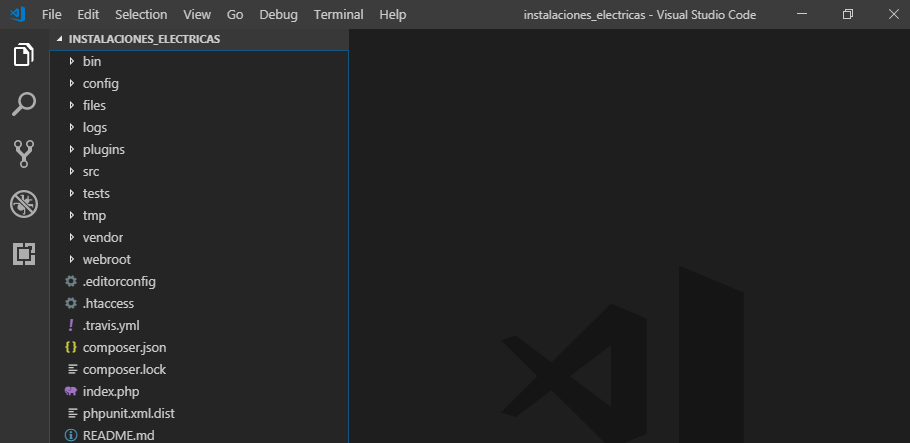
\includegraphics[width=1\textwidth]{/anexos/ManualProgramador/Xampp/7VscodeWeblectric}
	\caption{Estructura de directorios con el proyecto importado.}
	\label{img:VsCodeWeblectric}
\end{figure}

\newpage

Para acabar, en el archivo $app.conf$ que se encuentra dentro de la carpeta \textit{config}, es necesario reemplazar las lineas que a continuación se van a describir para enlazar el proyecto con la base de datos:

\begin{lstlisting}[language=php]
'Datasources' => [
	'default' => [
		'className' => 'Cake\Database\Connection',
		'driver' => 'Cake\Database\Driver\Mysql',
		'persistent' => false,
		'host' => 'localhost',
		'username' => 'Fran1234',
		'password' => 'Fran1234',
		'database' => 'weblectric',
		'encoding' => 'utf8',
		'timezone' => 'UTC',
		'flags' => [],
		'cacheMetadata' => true,
		'log' => false,
	],
],
\end{lstlisting}

\section{Despliegue en el servidor}

Como se ha comentado en secciones anteriores, la herramienta que se ha utilizado para establecer la conexión con el servidor ha sido \textit{Filezilla}. A través de esta herramienta, se realiza una conexión vía \textit{FTP} hacia la IP en la que se encuentra el servidor. En la figura~\ref{img:LoginFilezilla} se ve cómo establecer la conexión.

Para realizar el despliegue, solo hay que copiar el proyecto en la ruta adecuada. En este caso, ha de ser dentro del directorio \textit{httpdocs} como queda reflejado en la figura~\ref{img:Directorios}.

\begin{figure}[h]
	\centering
	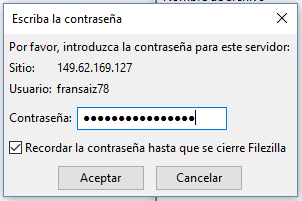
\includegraphics[width=0.6\textwidth]{/anexos/ManualProgramador/DespliegueServidor/LoginFilezilla}
	\caption{Acceso vía FTP al servidor.}
	\label{img:LoginFilezilla}
\end{figure}

\begin{figure}[h]
	\centering
	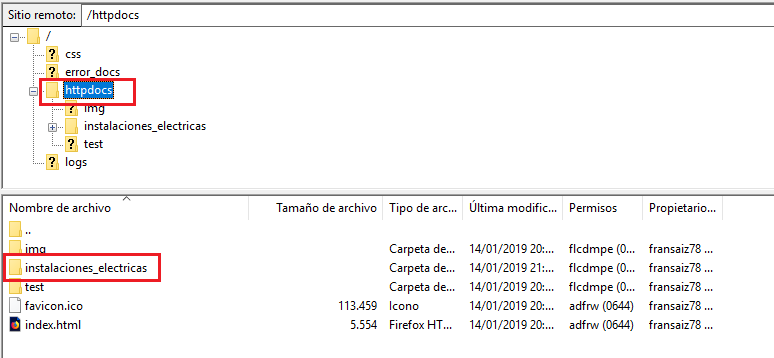
\includegraphics[width=1\textwidth]{/anexos/ManualProgramador/DespliegueServidor/Directorios}
	\caption{Estructura de directorios donde dejar la estructura del proyecto.}
	\label{img:Directorios}
\end{figure}



